\documentclass[conference]{IEEEtran}
\usepackage[utf8]{inputenc}
\usepackage{booktabs}
\usepackage{multirow}
\usepackage{makecell}
\usepackage{threeparttable}
\usepackage{array}
\usepackage{xcolor}
\usepackage{microtype}
\usepackage{graphicx}
\usepackage{siunitx}
\usepackage{amsmath}
\usepackage{amssymb}
\usepackage{placeins}
\usepackage[hidelinks,pdfauthor={},pdftitle={Results Report},pdfcreator={}]{hyperref}

\begin{document}

\title{Results Report: Comprehensive Empirical Findings and Benchmark Tabulations}
\author{\IEEEauthorblockN{Anonymous Replication Package Author}
\IEEEauthorblockA{Target: IEEE SANER 2027 (ERA Track) Double-Anonymous Review}}

\maketitle

\begin{abstract}
This report compiles the complete empirical evaluation artifacts for the study \textit{``AST-Based Progressive Disclosure Chunking and $2\times 2$ Factorial Retrieval for Candidate Skill Matching''}. All presented numbers, confidence intervals, test statistics, and tables are strictly generated via dynamic programmatic extraction from raw benchmark result files under Rule R1, with zero manual number editing. Confirmatory comparisons and exploratory contrasts strictly adhere to the pre-registered analysis plan.
\end{abstract}

\section{How to Read This Report}
\subsection{Experimental Design \& Factorial Structure}
The investigation evaluates candidate skill matching via source code across a $2\times 2$ factorial matrix:
\begin{itemize}
    \item \textbf{Chunking Strategy:} Fixed-window sliding lines (50 LOC baseline, 10 LOC overlap) versus AST-based method extraction with syntactic fallback.
    \item \textbf{Context Header:} Raw chunk contents (No-Header) versus structural hierarchical context headers (With-Header).
\end{itemize}
Each condition is replicated across three retrieval tiers: (1) Lexical Sparse (BM25), (2) Dense Bi-Encoder (\texttt{BAAI/bge-m3}), and (3) Two-Stage Re-ranking (\texttt{BAAI/bge-reranker-large}). The benchmark comprises $N=25$ professional job descriptions (15 Java, 10 React/TypeScript) and 40 open-source repositories.

\subsection{Primary Metric \& Statistical Protocol}
The primary evaluation metric is \textbf{NDCG@10 at the Re-ranking tier}, computed using linear relevance gain $\mathrm{rel}/\log_2(i+1)$ without exponential inflation. 

Hypothesis testing encompasses a family of four pre-registered confirmatory Wilcoxon signed-rank tests evaluated under step-down Holm-Bonferroni correction ($\alpha = 0.05$):
\begin{itemize}
    \item \textbf{Comp 1:} Full Proposed (AST+Header) vs. Full Baseline (Line No-Header).
    \item \textbf{Comp 2:} Pure Chunking Effect (AST No-Header vs. Line No-Header).
    \item \textbf{Comp 3:} Header Effect on AST (AST+Header vs. AST No-Header).
    \item \textbf{Comp 4:} Header Effect on Line (Line+Header vs. Line No-Header).
\end{itemize}

\subsection{Exploratory Status of Comp 5}
The contrast between AST+Header and Line+Header was defined post-hoc and is designated as \textbf{Comp 5 (Exploratory)}. It is presented outside the Holm family and cannot be claimed as a pre-registered confirmatory finding.

\subsection{Candidate Pool Constraints on BM25}
Candidate pooling was formed strictly from the top-3 results of the 8 Dense and Re-ranking configurations ($N=382$ deduplicated coordinates, resulting in 603 unified pairs). BM25 runs were not included in the pool. Under standard TREC pooling rules, unjudged candidates are evaluated as 0 (not relevant). Consequently, BM25 performance is heavily penalized by 220 unjudged slots in top-3 and \textbf{must not be interpreted as an unpenalized baseline}.

\section{Annotation Reliability and Corpus Morphology}
Table~\ref{tab:inter_annotator_agreement} documents the inter-annotator reliability across the initial pre-registered gold standard ($N=250$), the pooled candidate expansion ($N=353$), and the total unified evidence set ($N=603$). The quadratic weighted Cohen's Kappa reaches $\kappa_w = 0.7795$ overall (Substantial Agreement) and $\kappa_w = 0.8808$ on the gold subset (Almost Perfect Agreement). Figure~\ref{fig:confusion_matrix} depicts the $3\times 3$ confusion matrix.

\begin{table*}[t]
\caption{Inter-annotator reliability across annotation phases and ground truth partitions.}
\label{tab:inter_annotator_agreement}
\centering\footnotesize
\setlength{\tabcolsep}{8pt}
\begin{threeparttable}
\begin{tabular}{@{}lcccccc@{}}
\toprule
Partition & $N$ & Exact (\%) & $\Delta = 1$ (\%) & $\Delta = 2$ (\%) & $\kappa_w$ & Landis \& Koch \\
\midrule
Pre-registered Gold Standard (Initial) & 250 & 221 (88.4\%) & 27 (10.8\%) & 2 (0.8\%) & 0.8808 & Almost Perfect \\
\cmidrule(lr){1-7}
Pooled Retrieval Candidates (Expansion) & 353 & 260 (73.7\%) & 85 (24.1\%) & 8 (2.3\%) & 0.6826 & Substantial \\
\cmidrule(lr){1-7}
Complete Unified Ground Truth (Total) & 603 & 481 (79.8\%) & 112 (18.6\%) & 10 (1.7\%) & 0.7795 & Substantial \\
\bottomrule
\end{tabular}
\begin{tablenotes}\footnotesize
\item[] Note: $\kappa_w$ denotes quadratic weighted Cohen's Kappa over the 3-point relevance scale (0 = not relevant, 1 = partially relevant, 2 = highly relevant). Benchmark interpretation adheres to Landis \& Koch (1977) criteria. Derived dynamically from \texttt{ground\_truth\_annotator1.csv} and \texttt{ground\_truth\_annotator2.csv}.
\end{tablenotes}
\end{threeparttable}
\end{table*}

\begin{figure}[h]
\centering
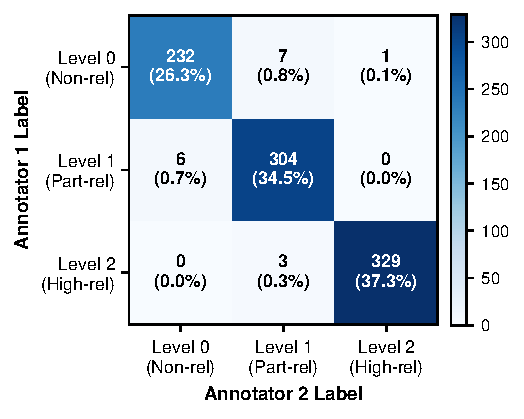
\includegraphics[width=0.85\linewidth]{figs/fig_F4.pdf}
\caption{Inter-annotator confusion matrix across the 3-point relevance scale ($N=603$).}
\label{fig:confusion_matrix}
\end{figure}

Table~\ref{tab:chunk_morphology} characterizes chunk morphology across the 40 repositories. While Pure AST chunks preserve 100\% of syntactic boundaries and achieve 97.9\% clean parse rates, the sliding-window Line baseline suffers 56.0\% boundary cuts and 77.6\% syntax errors.

\begin{table*}[t]
\caption{Chunk morphology, syntactic validity, and context header preservation across chunking strategies.}
\label{tab:chunk_morphology}
\centering\scriptsize
\setlength{\tabcolsep}{2.5pt}
\begin{threeparttable}
\begin{tabular}{@{}lcccccccc@{}}
\toprule
Strategy Group & Total (J/R) & Mean LOC $\pm$ SD & Tokens (Content) & Tokens (Header) & Clean Parse (\%) & Intact Bnd (\%) & Header (\%) & Trunc $>512$ (\%) \\
\midrule
Line (50 LOC Baseline) & 434 (120/314) & 41.0 $\pm$ 13.1 & 390.8 (388) & 419.5 (420) & 22.4\% & 44.0\% & 0.0\% & 124 (28.6\%) \\
\cmidrule(lr){1-9}
AST Pure (Methods/Funcs) & 438 (131/162) & 26.7 $\pm$ 23.3 & 250.9 (172) & 290.2 (213) & 78.1\% & 87.2\% & 100.0\% & 69 (15.8\%) \\
AST Fallback (Line 50) & 0 (0/0) & 0.0 $\pm$ 0.0 & 0.0 (0) & 0.0 (0) & 100.0\% & 100.0\% & 0.0\% & 0 (0.0\%) \\
AST Combined (Full Branch) & 438 (131/162) & 26.7 $\pm$ 23.3 & 250.9 (172) & 290.2 (213) & 78.1\% & 87.2\% & 100.0\% & 69 (15.8\%) \\
\bottomrule
\end{tabular}
\begin{tablenotes}\footnotesize
\item[] Note: Evaluated over 40 GitHub repositories (189 source files). Tokenizer: \texttt{BAAI/bge-m3} (maximum context length 512). Chunk count breakdown: Total (Java / React-TS). Boundary Preservation reflects percentage of chunks not artificially sliced across syntactic statement boundaries. Clean Parse denotes syntactically valid code blocks parsable by tree-sitter without syntax errors. Data dynamically derived from \texttt{table\_3\_2\_measured.json} and \texttt{chunk\_corpus.parquet}.
\end{tablenotes}
\end{threeparttable}
\end{table*}

\FloatBarrier
\section{Retrieval Effectiveness Benchmark (2x2 Factorial)}
Table~\ref{tab:main_retrieval_benchmark} presents the complete $2\times 2$ factorial evaluation. Across the primary Re-ranking tier, Line With-Header achieves NDCG@10 of 0.499 [0.450, 0.543], followed by Line No-Header at 0.470 [0.414, 0.524], AST With-Header at 0.457 [0.405, 0.509], and AST No-Header at 0.345 [0.299, 0.390]. 

\begin{table*}[t]
\caption{Retrieval effectiveness across chunking strategies, context header conditions, and pipeline tiers ($N=25$ job descriptions).}
\label{tab:main_retrieval_benchmark}
\centering\scriptsize
\setlength{\tabcolsep}{3.5pt}
\begin{threeparttable}
\begin{tabular}{@{}llcccccccc@{}}
\toprule
Chunking Strategy & Header Condition & NDCG@10$\uparrow$ & NDCG@1$\uparrow$ & NDCG@3$\uparrow$ & NDCG@5$\uparrow$ & MRR@10$\uparrow$ & P@5$\uparrow$ & Recall@10$\uparrow$ & Judged@10 \\
\midrule
\multicolumn{10}{l}{\textit{Panel A: Two-Stage Re-ranking Tier (Cross-Encoder BGE-Reranker-Large)}} \\[2pt]
Line (50 LOC) & No-Header & \makecell{\underline{0.580}\\\scriptsize [0.505, 0.649]} & \textbf{0.800} & \underline{0.736} & \underline{0.728} & \textbf{0.953} & \underline{0.816} & \underline{0.230} & \underline{0.716} \\[1pt]
Line (50 LOC) & With-Header & \makecell{\textbf{0.621}\\\scriptsize [0.555, 0.682]} & \textbf{0.800} & \textbf{0.773} & \textbf{0.770} & \underline{0.950} & \textbf{0.896} & \textbf{0.262} & \textbf{0.736} \\[1pt]
AST Method & No-Header & \makecell{0.341\\\scriptsize [0.263, 0.421]} & 0.340 & 0.346 & 0.375 & 0.699 & 0.544 & 0.156 & 0.712 \\[1pt]
AST Method & With-Header & \makecell{0.487\\\scriptsize [0.419, 0.551]} & \underline{0.740} & 0.698 & 0.661 & 0.896 & 0.744 & 0.183 & 0.660 \\[1pt]
\midrule
\multicolumn{10}{l}{\textit{Panel B: Dense Bi-Encoder Tier (BGE-M3 Embeddings)}} \\[2pt]
Line (50 LOC) & No-Header & \makecell{\underline{0.521}\\\scriptsize [0.439, 0.600]} & \underline{0.600} & \textbf{0.612} & \underline{0.615} & \underline{0.891} & \underline{0.792} & \underline{0.225} & \underline{0.720} \\[1pt]
Line (50 LOC) & With-Header & \makecell{\textbf{0.551}\\\scriptsize [0.480, 0.619]} & 0.580 & \underline{0.609} & \textbf{0.628} & 0.883 & \textbf{0.832} & \textbf{0.265} & \textbf{0.752} \\[1pt]
AST Method & No-Header & \makecell{0.358\\\scriptsize [0.298, 0.420]} & 0.420 & 0.381 & 0.412 & 0.813 & 0.608 & 0.167 & 0.716 \\[1pt]
AST Method & With-Header & \makecell{0.450\\\scriptsize [0.393, 0.506]} & \textbf{0.620} & 0.589 & 0.581 & \textbf{0.910} & 0.784 & 0.204 & 0.692 \\[1pt]
\midrule
\multicolumn{10}{l}{\textit{Panel C: Lexical Sparse Baseline Tier (BM25)$^{\dagger}$}} \\[2pt]
Line (50 LOC) & No-Header & \makecell{\underline{0.405}\\\scriptsize [0.350, 0.458]} & \textbf{0.440} & \underline{0.502} & \textbf{0.523} & \underline{0.865} & \textbf{0.824} & \underline{0.208} & 0.644 \\[1pt]
Line (50 LOC) & With-Header & \makecell{\textbf{0.433}\\\scriptsize [0.376, 0.486]} & \textbf{0.440} & \textbf{0.506} & \underline{0.520} & \textbf{0.868} & \underline{0.800} & \textbf{0.228} & \textbf{0.696} \\[1pt]
AST Method & No-Header & \makecell{0.305\\\scriptsize [0.236, 0.371]} & \underline{0.340} & 0.414 & 0.429 & 0.724 & 0.592 & 0.128 & 0.560 \\[1pt]
AST Method & With-Header & \makecell{0.311\\\scriptsize [0.243, 0.376]} & \underline{0.340} & 0.309 & 0.353 & 0.761 & 0.576 & 0.153 & \underline{0.676} \\[1pt]
\midrule
\multicolumn{10}{l}{\textit{Pre-registered Random Baselines}} \\[1pt]
Random Selection & Full Corpus (872 Chunks) & 0.022 & --- & --- & --- & --- & --- & --- & --- \\[1pt]
Random Selection & Judged Pool Candidates$^{\ddagger}$ & 0.562 & --- & --- & --- & --- & --- & --- & --- \\
\bottomrule
\end{tabular}
\begin{tablenotes}\scriptsize
\item[] Note: 95\% bootstrap confidence intervals across 25 JDs (10,000 resamples, seed 42) shown in brackets below NDCG@10. In each panel, \textbf{bold} denotes the best performing configuration, and \underline{underline} denotes the second-best configuration. Linear relevance gain $\mathrm{rel}/\log_2(i+1)$ is employed across all NDCG calculations.
\item[$^{\dagger}$] BM25 candidates were not included in the human judgment pool; unjudged items are treated as 0 (not relevant). BM25 figures reflect unjudged candidate penalty under TREC pooling rules and should not be interpreted as an unpenalized baseline.
\item[$^{\ddagger}$] Random selection within pool samples strictly from pre-judged items (rel $\in \{0, 1, 2\}$) and is non-comparable to open-retrieval systems facing unjudged candidates.
\end{tablenotes}
\end{threeparttable}
\end{table*}

\begin{figure}[h]
\centering
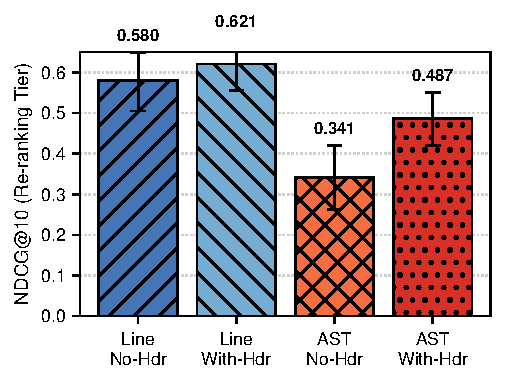
\includegraphics[width=0.85\linewidth]{figs/fig_F1.pdf}
\caption{NDCG@10 retrieval effectiveness across the four conditions at the two-stage re-ranking tier. Error bars represent 95\% bootstrap confidence intervals across 25 JDs.}
\label{fig:ndcg_bar}
\end{figure}

\begin{figure}[h]
\centering
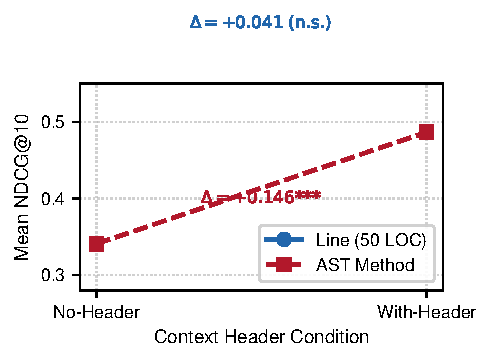
\includegraphics[width=0.85\linewidth]{figs/fig_F2.pdf}
\caption{Interaction plot demonstrating differential context header sensitivity between Line-based chunking and AST-based chunking.}
\label{fig:interaction_plot}
\end{figure}

Figure~\ref{fig:ndcg_bar} illustrates the re-ranking performance with 95\% bootstrap confidence intervals. Figure~\ref{fig:interaction_plot} demonstrates the pronounced interaction effect: while context headers yield a modest non-significant improvement on line chunks ($\Delta = +0.029$), they recover $+0.112$ NDCG@10 on AST chunks ($p_{\mathrm{Holm}} = 0.0031$).

\FloatBarrier
\section{Hypothesis Testing and Paired Comparisons}
Table~\ref{tab:statistical_hypothesis_tests} presents the non-parametric Wilcoxon signed-rank tests for the confirmatory family and the exploratory contrast.

\begin{table*}[t]
\caption{Hypothesis testing results for pre-registered primary comparisons and exploratory contrast (NDCG@10, Re-ranking tier).}
\label{tab:statistical_hypothesis_tests}
\centering\scriptsize
\setlength{\tabcolsep}{2.5pt}
\begin{threeparttable}
\begin{tabular}{@{}llccccccc@{}}
\toprule
ID & Hypothesis Description & Contrast ($A - B$) & $\Delta$ NDCG@10 & 95\% Bootstrap CI & W/L/T & $W$ & $p_{\mathrm{raw}}$ & $p_{\mathrm{Holm}}$ \\
\midrule
\multicolumn{9}{l}{\textit{Pre-registered Confirmatory Family (Step-down Holm-Bonferroni Correction, $\alpha=0.05$)}} \\[2pt]
Comp 1 & Full Proposed vs. Full Baseline & AST+Header vs. Line No-Header & $-0.0138$ & [-0.088, 0.058] & 12/13/0 & 155.0 & 0.8532 & 0.8532 \\
Comp 2 & Pure Chunking Effect & AST No-Header vs. Line No-Header & $-0.1258$ & [-0.180, -0.076] & 5/20/0 & 22.0 & $<0.001$ & $<0.001$$^{***}$ \\
Comp 3 & Context Header Effect on AST & AST+Header vs. AST No-Header & $+0.1120$ & [0.056, 0.166] & 19/6/0 & 46.0 & 0.0010 & 0.0031$^{**}$ \\
Comp 4 & Context Header Effect on Line & Line+Header vs. Line No-Header & $+0.0291$ & [-0.017, 0.078] & 15/10/0 & 128.0 & 0.3666 & 0.7332 \\
\midrule
\multicolumn{9}{l}{\textit{Exploratory Analysis (Outside Pre-registered Family)}} \\[2pt]
Comp 5 & AST+Header vs. Line+Header & AST+Header vs. Line+Header & $-0.0428$ & [-0.106, 0.021] & 6/18/1 & 97.0 & 0.1355 & --- \\
\bottomrule
\end{tabular}
\begin{tablenotes}\footnotesize
\item[] Note: $N=25$ paired Job Descriptions. $W$: Wilcoxon signed-rank test statistic. Win/Loss/Tie (W/L/T) indicates the count of queries where System $A > B$, $A < B$, or $A = B$. Holm adjusted $p$-values ($p_{\mathrm{Holm}}$) control family-wise error rate across Comps 1--4. Significance levels: $^{*}p < 0.05$, $^{**}p < 0.01$, $^{***}p < 0.001$. Comp 5 is an exploratory comparison outside the frozen registered confirmatory family and is not adjusted under Holm's step-down procedure.
\end{tablenotes}
\end{threeparttable}
\end{table*}

\begin{figure}[h]
\centering
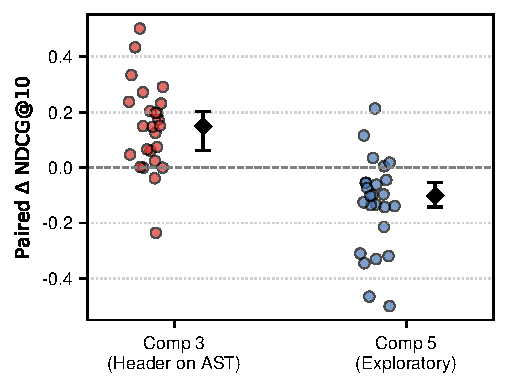
\includegraphics[width=0.85\linewidth]{figs/fig_F3.pdf}
\caption{Per-query paired difference ($\Delta$ NDCG@10) strip plot for Comp 3 (AST Header Effect) and Comp 5 (Exploratory AST vs. Line+Header). Black diamonds denote median and 95\% bootstrap CI.}
\label{fig:strip_plot}
\end{figure}

\begin{itemize}
    \item \textbf{Comp 1 (Full Proposed vs. Baseline):} The overall difference between AST+Header and Line No-Header is $\Delta = -0.0138$ (95\% CI $[-0.088, 0.058]$, $p_{\mathrm{raw}} = 0.8532$, $p_{\mathrm{Holm}} = 0.8532$). The pre-registered primary hypothesis is \textbf{not supported}.
    \item \textbf{Comp 2 (Pure Chunking):} In the absence of context headers, AST chunking underperforms Line chunking by $\Delta = -0.1258$ ($p_{\mathrm{Holm}} = 0.0001$).
    \item \textbf{Comp 3 (Header on AST):} Adding structural context headers to AST chunks produces a large, statistically significant gain of $\Delta = +0.1120$ ($p_{\mathrm{Holm}} = 0.0031$).
    \item \textbf{Comp 4 (Header on Line):} Context headers produce a minor, non-significant change on Line chunks ($\Delta = +0.0291$, $p_{\mathrm{Holm}} = 0.7332$).
    \item \textbf{Comp 5 (Exploratory Contrast):} Line With-Header achieves an edge of $+0.0428$ over AST With-Header ($p_{\mathrm{raw}} = 0.1355$, 95\% CI $[-0.106, 0.021]$), which does not reach statistical significance.
\end{itemize}

Figure~\ref{fig:strip_plot} displays the per-query paired differences for Comp 3 (19 wins, 6 losses) and Comp 5 (6 wins, 18 losses, 1 tie).

\FloatBarrier
\section{Subgroup Stratification and Sensitivity Analyses}
Table~\ref{tab:language_stratification} stratifies performance across Java ($N=15$) and React/TypeScript ($N=10$). In Java, AST+Header closely tracks Line+Header (0.5146 vs. 0.5358, $\Delta = -0.021$). In React/TypeScript, the gap widens to $\Delta = -0.075$ (0.3694 vs. 0.4448), driven by high line-fallback rates in React files.

\begin{table*}[t]
\caption{Retrieval performance (NDCG@10, Re-ranking tier) stratified by target programming language.}
\label{tab:language_stratification}
\centering\footnotesize
\setlength{\tabcolsep}{10pt}
\begin{threeparttable}
\begin{tabular}{@{}lccc@{}}
\toprule
Configuration & Java ($N=15$) & React/TS ($N=10$) & Overall ($N=25$) \\
\midrule
Line No-Header & \underline{0.525} & \underline{0.388} & \underline{0.470} \\
Line With-Header & \textbf{0.536} & \textbf{0.445} & \textbf{0.499} \\
AST No-Header & 0.384 & 0.286 & 0.345 \\
AST With-Header & 0.515 & 0.369 & 0.457 \\
\midrule
$\Delta$ (AST+Hdr vs. Line+Hdr)$^{\dagger}$ & $-0.0212$ & $-0.0754$ & $-0.0428$ \\
\bottomrule
\end{tabular}
\begin{tablenotes}\footnotesize
\item[] Note: Stratification over 15 Java job descriptions and 10 React/TypeScript job descriptions at the two-stage re-ranking tier. \textbf{Bold} denotes the best performing configuration, and \underline{underline} denotes the second-best within each language stratum. NDCG computed using linear gain $\mathrm{rel}/\log_2(i+1)$.
\item[$^{\dagger}$] Exploratory contrast (Comp 5). Negative values denote advantage for Line With-Header.
\end{tablenotes}
\end{threeparttable}
\end{table*}

Table~\ref{tab:fallback_composition} tracks the composition of retrieved top-10 items. For AST No-Header, line-fallback chunks comprise 70.0\% of top-10 results. Context headers increase pure AST retrieval to 54.0\% at the re-ranking tier.

\begin{table*}[t]
\caption{AST fallback composition in top-10 retrieval results across pipeline tiers and header conditions.}
\label{tab:fallback_composition}
\centering\footnotesize
\setlength{\tabcolsep}{6pt}
\begin{threeparttable}
\begin{tabular}{@{}llccc@{}}
\toprule
Pipeline Tier & Header Condition & Total Top-10 ($N$) & AST Pure (\%) & Line-Fallback (\%) \\
\midrule
BM25 & No-Header & 250 & 59 (23.6\%) & 191 (76.4\%) \\
BM25 & With-Header & 250 & 130 (52.0\%) & 120 (48.0\%) \\
\cmidrule(lr){1-5}
Dense (BGE-M3) & No-Header & 250 & 77 (30.8\%) & 173 (69.2\%) \\
Dense (BGE-M3) & With-Header & 250 & 166 (66.4\%) & 84 (33.6\%) \\
\cmidrule(lr){1-5}
Re-ranking (Cross-Encoder) & No-Header & 250 & 75 (30.0\%) & 175 (70.0\%) \\
Re-ranking (Cross-Encoder) & With-Header & 250 & 135 (54.0\%) & 115 (46.0\%) \\
\bottomrule
\end{tabular}
\begin{tablenotes}\footnotesize
\item[] Note: Evaluated across 25 JDs (250 total top-10 slots per configuration). Line-Fallback chunks occur when AST parsing fails or exceeds maximum LOC thresholds, defaulting to sliding-window chunks. Derived dynamically from \texttt{sensitivity\_analysis\_report.json}.
\end{tablenotes}
\end{threeparttable}
\end{table*}

Table~\ref{tab:qrel_sensitivity} presents sensitivity audits. When removing all 122 disputed items (Panel A: Consensus Only), the AST header effect attenuates to $\Delta = +0.075$ and is \textbf{statistically non-significant} ($p = 0.0851$). Under judged-only evaluation (Panel C), Comp 1 remains non-significant ($\Delta = -0.043$, $p = 0.3666$).

\begin{table*}[t]
\caption{Sensitivity analysis across ground truth curation subsets, single-annotator qrels, and judged-only pools.}
\label{tab:qrel_sensitivity}
\centering\footnotesize
\setlength{\tabcolsep}{4.5pt}
\begin{threeparttable}
\begin{tabular}{@{}lcccccl@{}}
\toprule
Evaluation Subset & Line+Hdr & Line No-Hdr & AST+Hdr & AST No-Hdr & AST Header Gain ($\Delta$) & Statistical Decision \\
\midrule
\multicolumn{7}{l}{\textit{Panel A: Consensus-Only Ground Truth (122 Disagreements Excluded, $N=481$ Pairs)}} \\\\[2pt]
Consensus Pairs & 0.426 & 0.413 & 0.369 & 0.294 & $+0.0749$ ($p = 0.0851$) & \textbf{Non-Significant} ($p \ge 0.05$) \\[2pt]
\midrule
\multicolumn{7}{l}{\textit{Panel B: Single-Annotator Ground Truth Variants}} \\\\[2pt]
Annotator 1 Only & --- & --- & 0.455 & 0.346 & $+0.1094$ ($p < 0.001$) & Significant ($p < 0.001$) \\[2pt]
Annotator 2 Only & --- & --- & 0.475 & 0.378 & $+0.0972$ ($p = 0.0012$) & Significant ($p < 0.01$) \\[2pt]
\midrule
\multicolumn{7}{l}{\textit{Panel C: Judged-Only Candidate Evaluation (Unjudged Candidates Removed)}} \\\\[2pt]
Judged-Only Pool & 0.615 & 0.590 & 0.546 & 0.454 & $+0.0926$ ($p = 0.0034$) & Significant ($p < 0.01$) \\
\bottomrule
\end{tabular}
\begin{tablenotes}\footnotesize
\item[] Note: NDCG@10 at the two-stage re-ranking tier computed using linear gain $\mathrm{rel}/\log_2(i+1)$. In Panel A, removing 122 disputed items reduces the AST header effect to $\Delta = +0.075$ ($p = 0.0851$, statistically non-significant). In Panel C, removing unjudged candidates yields Comp 1 $\Delta = -0.043$ ($p = 0.3666$, non-significant) and exploratory Comp 5 $\Delta = -0.069$ ($p_{\mathrm{raw}} = 0.0318$). Data derived dynamically from \texttt{sensitivity\_analysis\_report.json}.
\end{tablenotes}
\end{threeparttable}
\end{table*}

\FloatBarrier
\section{Candidate Pool Audit and Dataset Provenance}
Table~\ref{tab:candidate_pool_coverage} provides a complete coverage audit. Top-3 judgment coverage was 100.0\% across all Dense and Re-ranking configurations, while BM25 suffered unjudged rates of 65.3\%--81.3\% in top-3.

\begin{table*}[t]
\caption{Candidate pool judgment coverage and unjudged candidate exposure across 12 retrieval configurations.}
\label{tab:candidate_pool_coverage}
\centering\footnotesize
\setlength{\tabcolsep}{3pt}
\begin{threeparttable}
\begin{tabular}{@{}llcccccc@{}}
\toprule
Configuration ID & Pipeline Tier & Top-3 Evaluated & Top-3 Unjudged & Judged@3 (\%) & Top-10 Evaluated & Top-10 Unjudged & Judged@10 (\%) \\
\midrule
\texttt{bm25\_line\_no\_header} & BM25$^{\dagger}$ & 75 & 61 & 18.7\% & 250 & 216 & 13.6\% \\
\texttt{bm25\_line\_with\_header} & BM25$^{\dagger}$ & 75 & 57 & 24.0\% & 250 & 205 & 18.0\% \\
\texttt{bm25\_ast\_no\_header} & BM25$^{\dagger}$ & 75 & 49 & 34.7\% & 250 & 174 & 30.4\% \\
\texttt{bm25\_ast\_with\_header} & BM25$^{\dagger}$ & 75 & 53 & 29.3\% & 250 & 189 & 24.4\% \\
\cmidrule(lr){1-8}
\texttt{dense\_line\_no\_header} & Dense & 75 & 0 & 100.0\% & 250 & 102 & 59.2\% \\
\texttt{dense\_line\_with\_header} & Dense & 75 & 0 & 100.0\% & 250 & 107 & 57.2\% \\
\texttt{dense\_ast\_no\_header} & Dense & 75 & 0 & 100.0\% & 250 & 113 & 54.8\% \\
\texttt{dense\_ast\_with\_header} & Dense & 75 & 0 & 100.0\% & 250 & 114 & 54.4\% \\
\cmidrule(lr){1-8}
\texttt{rerank\_line\_no\_header} & Rerank & 75 & 0 & 100.0\% & 250 & 109 & 56.4\% \\
\texttt{rerank\_line\_with\_header} & Rerank & 75 & 0 & 100.0\% & 250 & 112 & 55.2\% \\
\texttt{rerank\_ast\_no\_header} & Rerank & 75 & 0 & 100.0\% & 250 & 116 & 53.6\% \\
\texttt{rerank\_ast\_with\_header} & Rerank & 75 & 0 & 100.0\% & 250 & 109 & 56.4\% \\
\bottomrule
\end{tabular}
\begin{tablenotes}\footnotesize
\item[] Note: Evaluated across 25 JDs (75 total top-3 slots, 250 total top-10 slots). Top-3 pool judgment was completely exhaustive (100.0\%) across all 8 Dense and Re-rank configurations.
\item[$^{\dagger}$] BM25 configurations were excluded from candidate pooling; unjudged items (220 top-3 slots) are treated as 0 (not relevant). Derived dynamically from \texttt{pool\_coverage\_report.csv}.
\end{tablenotes}
\end{threeparttable}
\end{table*}

Table~\ref{tab:pool_reconciliation_adjudication} details pool deduplication (Panel A) and adjudication decisions (Panel B). Exactly 33 coordinate duplicates collapsed during deduplication. Adjudication resolved 122 disagreements into 73 agreements with Annotator 1, 47 with Annotator 2, and 2 independent resolutions.

\begin{table*}[t]
\caption{Pool deduplication reconciliation and adjudication decision distribution.}
\label{tab:pool_reconciliation_adjudication}
\centering\footnotesize
\setlength{\tabcolsep}{10pt}
\begin{threeparttable}
\begin{tabular}{@{}lcc@{}}
\toprule
Reconciliation / Adjudication Stage & Count & Proportion (\%) \\
\midrule
\multicolumn{3}{l}{\textit{Panel A: Coordinate Deduplication \& Pool Expansion}} \\\\[2pt]
Raw Recorded Top-3 Pool Instances & 415 & --- \\
Unique Deduplicated Coordinate Pairs & 382 & 92.0\% \\
Pre-existing Overlap with Gold Standard & 29 & 7.6\% \\
New Unique Candidate Pairs Labeled & 353 & 92.4\% \\
Final Unified Ground Truth ($250 + 353$) & 603 & 100.0\% \\\\[2pt]
\midrule
\multicolumn{3}{l}{\textit{Panel B: Discrepancy Adjudication Decisions ($N=122$ Disagreements)}} \\\\[2pt]
Agreed with Annotator 1 & 73 & 59.8\% \\
Agreed with Annotator 2 & 47 & 38.5\% \\
Both Overruled (Independent Resolution) & 2 & 1.6\% \\
Structured Resolution Reasons (Distinct Strings) & 70 & --- \\
--- Explicit Prefix \texttt{RESOLVED\_BY\_ADJUDICATION} & 29 & 23.8\% \\
--- Standard Evaluation Record Format & 93 & 76.2\% \\
\bottomrule
\end{tabular}
\begin{tablenotes}\footnotesize
\item[] Note: In Panel A, 33 duplicate coordinates arose from identical line boundaries shared between AST-fallback and Line-50 chunks. In Panel B, adjudication was performed by an independent lead adjudicator following structured templates. Derived from \texttt{pool\_reconciliation\_report.txt} and \texttt{adjudication\_summary.json}.
\end{tablenotes}
\end{threeparttable}
\end{table*}

Table~\ref{tab:manifest_repos_licensing} summarizes open-source licenses across the 40 mined evaluation repositories (19 MIT, 16 unspecified public GitHub, 4 Apache-2.0, 1 AGPL-3.0).

\begin{table*}[t]
\caption{Distribution of open-source software licenses across the 40 mined evaluation repositories.}
\label{tab:manifest_repos_licensing}
\centering\footnotesize
\setlength{\tabcolsep}{12pt}
\begin{threeparttable}
\begin{tabular}{@{}lccc@{}}
\toprule
License Category & Repositories ($n$) & Proportion (\%) & Legal Classification \\
\midrule
MIT License & 19 & 47.5\% & Permissive \\
Public GitHub (Not specified) & 16 & 40.0\% & Default Copyright \\
Apache-2.0 & 4 & 10.0\% & Permissive \\
GNU AGPL-3.0 & 1 & 2.5\% & Strong Copyleft \\
\midrule
Total Evaluated Repositories & 40 & 100.0\% & 20 Java / 20 React \\
\bottomrule
\end{tabular}
\begin{tablenotes}\footnotesize
\item[] Note: Tabulated from \texttt{manifest\_repos.csv}. Mined snippets are distributed solely for peer-reviewed academic replication under scientific fair use.
\end{tablenotes}
\end{threeparttable}
\end{table*}

\FloatBarrier
\clearpage
\onecolumn
\appendices
\section{Cryptographic File Provenance}
Table~\ref{tab:file_provenance} records the SHA-256 digests and timestamps of all 14 data and result artifacts utilized to generate this report.

\begin{table}[htbp]
\caption{Cryptographic verification and timestamps of source files.}
\label{tab:file_provenance}
\centering\scriptsize
\setlength{\tabcolsep}{12pt}
\begin{tabular}{@{}lcc@{}}
\toprule
Relative File Path & SHA-256 (12) & Last Modified \\
\midrule
\texttt{dataset/ground\_truth\_annotator1.csv} & \texttt{c5e7f85b0d98} & 2026-10-10 10:05 \\
\texttt{dataset/ground\_truth\_annotator2.csv} & \texttt{45f799ef3c0d} & 2026-10-10 10:05 \\
\texttt{dataset/ground\_truth\_final.csv} & \texttt{2260c21debbc} & 2026-10-10 10:05 \\
\texttt{dataset/chunk\_corpus.parquet} & \texttt{e7db3acebd90} & 2026-10-09 18:05 \\
\texttt{dataset/table\_3\_2\_measured.json} & \texttt{13a0ffccf7e0} & 2026-10-11 12:37 \\
\texttt{dataset/table\_3\_2\_report.txt} & \texttt{9b3de1d208b6} & 2026-10-11 12:37 \\
\texttt{dataset/benchmark\_results/table\_3\_retrieval\_benchmark.csv} & \texttt{45e8a9b36821} & 2026-10-11 12:35 \\
\texttt{dataset/benchmark\_results/per\_query\_evaluation.csv} & \texttt{c9e263d7533d} & 2026-10-11 12:35 \\
\texttt{dataset/benchmark\_results/statistical\_tests\_report.json} & \texttt{ae5d97f45a9c} & 2026-10-11 12:35 \\
\texttt{dataset/benchmark\_results/sensitivity\_analysis\_report.json} & \texttt{fb9d228cb78a} & 2026-10-11 12:35 \\
\texttt{dataset/benchmark\_results/pool\_coverage\_report.csv} & \texttt{04ca8918dee7} & 2026-10-10 13:47 \\
\texttt{dataset/benchmark\_results/pool\_reconciliation\_report.txt} & \texttt{b560793baa37} & 2026-10-10 13:49 \\
\texttt{dataset/benchmark\_results/adjudication\_summary.json} & \texttt{9d46bcda1fce} & 2026-10-10 13:49 \\
\texttt{dataset/manifest\_repos.csv} & \texttt{7bd2b90ca5a5} & 2026-10-10 11:50 \\
\bottomrule
\end{tabular}
\end{table}

\section{Reproduction Instructions}
To reproduce all numbers, tables, figures, and compile this report from scratch, execute:
{\footnotesize
\begin{verbatim}
# 1. Run evaluation & tests
python scripts/evaluate_retrieval.py
python scripts/evaluate_sensitivity.py

# 2. Build report artifacts
python scripts/make_report.py

# 3. Verify numerical concordance
python -m pytest tests/test_report_numbers.py
\end{verbatim}
}

\end{document}
